\documentclass[11pt]{beamer}
\usetheme{Singapore}
%\usecolortheme{dove}
\usepackage{etoolbox}
\usepackage{ragged2e}
\usepackage[utf8]{inputenc}
\usepackage[italian]{babel}
\usepackage{scrextend}
\usepackage{tikz}
\usepackage{adjustbox}
\usepackage{multirow}
\AtBeginSection[]{\frame{\Huge \centering \insertsection} \subsection{} }
%\AtBeginSection[]{\subsection{}}
\usetikzlibrary{shapes.geometric, arrows}
\tikzstyle{startstop} = [rectangle, 
rounded corners, 
minimum width=1cm, 
minimum height=.5cm,
text centered, 
draw=black, 
fill=red!30]

\tikzstyle{io} = [trapezium, 
trapezium left angle=70, 
trapezium right angle=110, 
minimum width=1cm, 
minimum height=0.5cm, 
text centered, 
draw=black, 
fill=blue!30
]
\tikzstyle{process} = [rectangle, 
minimum width=1cm, 
minimum height=.5cm, 
text centered, 
draw=black, 
fill=orange!30, 
text width=0.95\linewidth]

\tikzstyle{process_red} = [rectangle, 
minimum width=3cm, 
minimum height=1cm, 
text centered, 
draw=black, 
fill=red!70, 
text width=0.95\linewidth]

\tikzstyle{decision} = [diamond, 
minimum width=4cm, 
minimum height=4cm, 
text centered, 
draw=black, 
fill=green!30, 
text width= 3.5cm ]

\tikzstyle{arrow} = [thick,
->,
>=stealth]


\apptocmd{\frame}{}{\justifying}{}
\author{Cap. Alberto Azzalini}
\title[Analisi Forense]{Analisi forense\\Repertamento di materiale informatico}
\subtitle{Introduzione alle modalità operative}

%\logo{
\includegraphics[height=0.1\linewidth]{pics/stemma-della-repubblica-italiana-colori}}

\institute{Legione Carabinieri ``Trentino Alto Adige''\\Comando Provinciale di Bolzano\\Compagnia di Vipiteno}

\date{31 marzo 2016}

%subject{}

\setbeamercovered{transparent}

%\setbeamertemplate{navigation symbols}{}

\begin{document}
	\maketitle
	
	\begin{frame}
		\frametitle{Indice dei contenuti}
		\tableofcontents
	\end{frame}

	\section{Premessa}
	\begin{frame}
		\frametitle{I reati informatici}
%		\justifying
		Si possono distinguere:
		\begin{itemize}
			\item reati informatici propri;
			\item reati comuni con una componente informatica.
		\end{itemize}  
				
		Tuttavia ormai non esiste fenomeno giuridicamente rilevante che non abbia una componente digitale dalla quale estrarre informazioni utili alla ricostruzione dei fatti.
		\vfill
		Anche la ``semplice'' analisi di un tabulato telefonico è una analisi di natura informatica.
				
	\end{frame}
	
	\begin{frame}
		\frametitle{L'evoluzione dell'informatica forense}
			Le procedure operative sono notevolmente cambiate per rispondere alle esigenze connesse alle nuove tecnologie di comunicazione informatica e all'avvento dei \textit{social network}.
			\vfill
			Prima si staccava molto semplicemente la spina di un computer e lo si repertava: oggi invece si sa che il contenuto della memoria volatile può essere molto utile per le indagini e non può essere disperso.
	\end{frame}
	
	\begin{frame}
		\frametitle{Le regole del repertamento e dell'analisi forense}
		Gli operatori si dovrebbero attenere a poche, semplici regole, reperibili da varie fonti, tra cui (sopra tutte le altre) devono essere considerate:
		\begin{itemize}
			\item il Codice di Procedura Penale;
			\item il buon senso;
			\item il proprio intuito investigativo, maturato in anni di indagini, non necessariamente ad alta tecnologia;
			\item colleghi o tecnici di comprovata esperienza.
		\end{itemize}
		\vfill
		Nessun tecnico puro, nemmeno il più bravo, può sostituirsi all'investigatore nell'analizzare i dati ricavati da un sistema informatico: \textit{gli mancano la sensibilità e l'intuito dello sbirro!}
		
	\end{frame}
	
	
	\section{Fonti normative}
	\begin{frame}
		\frametitle{La legislazione italiana}
		La legge n.~48 del 18 marzo 2008\cite{L_48/2008_2016-03-04} ratifica la Convenzione del Consiglio d'Europa sulla criminalità informatica, risalente al novembre 2001:
		\begin{itemize}
			\item introduce significative modifiche al codice penale in ambito informatico;
			\item introduce novità al Codice di Procedura Penale interessanti per l'informatica forense.
		\end{itemize} 
	\end{frame}
	
	\begin{frame}[shrink]
		\frametitle{Le modifiche al Codice di Procedura Penale [1/4]}
%		\fontsize{8pt}{\baselineskip}\selectfont
		\begin{center}
			\textbf{Art.~244 c.p.p.} \\\textit{Casi e forme delle ispezioni}	
		\end{center}		
			\begin{labeling}{1.}
				\item[1.] L'ispezione delle persone, dei luoghi e delle cose è disposta con decreto motivato quando occorre accertare le tracce e gli altri effetti materiali del reato.
				\item[2.] Se il reato non ha lasciato tracce o effetti materiali, o se questi sono scomparsi o sono stati cancellati o dispersi, alterati o rimossi, l'autorità giudiziaria descrive lo stato attuale e, in quanto possibile, verifica quello preesistente, curando anche di individuare modo, tempo e cause delle eventuali modificazioni. L'autorità giudiziaria può disporre rilievi segnaletici, descrittivi e fotografici e ogni altra operazione tecnica [359], \textbf{anche in relazione a sistemi informatici o telematici, adottando misure tecniche dirette ad assicurare la conservazione dei dati originali e ad impedirne l'alterazione.}
			\end{labeling}
	\end{frame}
	\begin{frame}[shrink]
		\frametitle{Le modifiche al Codice di Procedura Penale [2/4]}
%		\fontsize{8pt}{\baselineskip}\selectfont
			\begin{center}
				\textbf{Art. 247 c.p.p.} \\\textit{Casi e forme delle perquisizioni}
			\end{center}
			\begin{labeling}{1-bis.}
				\item[ \textellipsis ]
				\item[1-bis.] Quando vi è fondato motivo di ritenere che dati, informazioni, programmi informatici o tracce comunque pertinenti al reato si trovino in un sistema informatico o telematico, ancorché protetto da misure di sicurezza, ne è disposta la perquisizione, adottando misure tecniche dirette ad assicurare la conservazione dei dati originali e ad impedirne l'alterazione.
				\item[\textellipsis]
			\end{labeling}
	\end{frame}
	\begin{frame}[shrink]
		\frametitle{Le modifiche al Codice di Procedura Penale [3/4]}
%		\fontsize{8pt}{\baselineskip}\selectfont
			\begin{center}
				\textbf{Art. 352 c.p.p.} \\\textit{Perquisizioni}
			\end{center}
			\begin{labeling}{1.bis.}
				\item[\textellipsis]
				\item[1-bis.] Nella flagranza del reato, ovvero nei casi di cui al comma 2 quando sussistono i presupposti e le altre condizioni ivi previsti, gli ufficiali di polizia giudiziaria, adottando misure tecniche dirette ad assicurare la conservazione dei dati originali e ad impedirne l'alterazione, procedono altresì alla perquisizione di sistemi informatici o telematici, ancorché protetti da misure di sicurezza, quando hanno fondato motivo di ritenere che in questi si trovino occultati dati, informazioni, programmi informatici o tracce comunque pertinenti al reato che possono essere cancellati o dispersi.
				\item[\textellipsis]
			\end{labeling}
	\end{frame}
	\begin{frame}[shrink]
		\frametitle{Le modifiche al Codice di Procedura Penale [4/4]}
%		\fontsize{8pt}{\baselineskip}\selectfont
			\begin{center}
				\textbf{Art. 354 c.p.p.}\\\textit{Accertamenti urgenti sui luoghi, sulle cose e sulle persone. Sequestro.}
			\end{center}
			\begin{labeling}{2.}
				\fontsize{7pt}{\baselineskip}\selectfont
				\setcounter{enumi}{1}
				\item[2.] Se vi è pericolo che le cose, le tracce e i luoghi indicati nel comma 1 si alterino o si disperdano o comunque si modifichino e il pubblico ministero non può intervenire tempestivamente, ovvero non ha ancora assunto la direzione delle indagini, gli ufficiali di polizia giudiziaria compiono i necessari accertamenti e rilievi sullo stato dei luoghi e delle cose. \textbf{In relazione ai dati, alle informazioni e ai programmi informatici o ai sistemi informatici o telematici, gli ufficiali della polizia giudiziaria adottano, altresì, le misure tecniche o impartiscono le prescrizioni necessarie ad assicurarne la conservazione e ad impedirne l'alterazione e l'accesso e provvedono, ove possibile, alla loro immediata duplicazione su adeguati supporti, mediante una procedura che assicuri la conformità della copia all'originale e la sua immodificabilità.} Se del caso, sequestrano il corpo del reato e le cose a questo pertinenti.
			\end{labeling}
	\end{frame}

	\begin{frame}
		\frametitle{Implicazioni della L. 48/2008 [1/2]}
		La legge 48 del 2008 ha introdotto nel codice di procedura penale:
		\begin{itemize}
		\item concetto di scena del crimine virtuale
		\item ispezioni e perquisizioni ``virtuali''
		\item concetto di copia conforme all'originale del dato informatico
		\item clausola dell'immodificabilità di quanto copiato.
		\end{itemize}		
		\vfill
		La 48/2008 impone di adottare misure tecniche che \textbf{assicurino la conservazione dei dati originali e ne impediscano l'alterazione}.
		\vfill
		Infatti, ogni intervento su un sistema informatico  condotto in maniera \textbf{non forense} comporta sempre e comunque un'alterazione dei dati e spesso anche la cancellazione di parte di essi.
	\end{frame}
	\begin{frame}
		\frametitle{Implicazioni della L. 48/2008 [2/2]}	
		Nel dettaglio, le fasi standard dell'indagine digitale forense sono:
		\begin{enumerate}
			\item identificazione e prelievo;
			\item preservazione e archiviazione;
			\item analisi tecnica e investigativa;
			\item reporting tecnico e legale.
		\end{enumerate}
		\vfill
		Qui si approfondiranno le procedure di identificazione e prelievo, trattando in maniera più rapida quelle relative agli altri tre aspetti, che di norma sono di competenza di organi e reparti specializzati o di personale in possesso di competenze specifiche.
	\end{frame}
	
	\section[Repertamento]{I principi del repertamento}
	
	\begin{frame}
		\frametitle{In un mondo perfetto\dots}
		Le attività di repertamento dovrebbero essere svolte da personale specializzato: già in sede di sopralluogo è necessario evitare errori e operare con cognizione di causa, soprattutto se diventa necessario analizzare immediatamente le apparecchiature accese.
		\vfill
		Nella maggior parte dei casi interviene personale del pronto intervento, della stazione o, se si è fortunati, del Reparto Operativo (che comunque non sempre ha una preparazione specifica -- e il collega che ce l'ha è in licenza). 
		\vfill
		\'{E} quindi fondamentale che \textbf{ogni operatore} abbia almeno un'idea di base su come procedere al meglio.
	\end{frame}
	
	\begin{frame}
		\frametitle{Procedure operative per il repertamento digitale}
		Possiamo distinguere due tipi di repertamento di un sistema digitale:
		
		\begin{itemize}
			\item \textbf{il repertamento dell'oggetto fisico}, che mantiene i dati seguendo un qualche principio fisico (in genere elettrico, magnetico e/o ottico);
			\item \textbf{il repertamento dei dati} ossia la fedele copia dei dati su supporto sicuro.
		\end{itemize}
		\vfill
		Normalmente il primo precede il secondo, che viene effettuato in laboratorio. \textbf{La 48/2008 dà però anche la possibilità di procedere in loco alla copia dei dati o alla loro immediata visualizzazione}. Si parla in questo caso di \textit{live forensic}.
		
	\end{frame}
	
	\begin{frame}
		\frametitle{Fissare le priorità}
		Indipendentemente dalla presenza o meno di tecnologie informatiche, la scena del crimine è un \textit{puzzle} che l'investigatore deve riuscire a ricomporre. 
		\vfill
		Poiché è impossibile analizzare ogni singolo elemento, si devono stabilire delle priorità in base a:
		\begin{itemize}
			\item tipologia di reato;
			\item tipologia di reperti;
			\item tipo di informazioni che cerchiamo;
			\item profilo dell'indagato/sospettato.
		\end{itemize}
		\vfill
		Di questa ``analisi delle priorità'' dovremo tenere conto sia in fase di sopralluogo e di raccolta del materiale, sia in fase di esame tecnico forense.
	\end{frame}
	\begin{frame}
		\frametitle{Sequenza delle operazioni}
		\begin{adjustbox}{max totalsize={\textwidth}{\textheight},center,valign=M}
			\Large
			\begin{tikzpicture}[node distance=1.8cm]
			
			\node (start) [startstop, text width=15cm ] {Individuare il computer o il dispositivo da sequestrare};
			
			\node (pro1) [process, below of=start, text width=18cm, yshift=0.3cm ] {Mettere in sicurezza l'area e la scena del delitto facendo allontanare gli estranei dalle apparecchiature e dai quadri elettrici};
			
			\node (dec1) [decision, below of=pro1, yshift=-0.7cm, xshift=-10cm, text width=3cm ] {Il bersaglio è acceso?};
			
			\node (dec2) [decision, right of=dec1, xshift=19cm, text width=3cm] {C'è un esperto a disposizione?};
			
			\node (pro2) [process_red, below of=dec1, yshift=-4.2cm, text width=4cm] {NON ACCENDERLO!};
			
			\node (pro3) [process_red, below of=dec2, text width=4cm,  yshift=-4.2cm] {Seguire i suoi consigli};
			
			\node (pro4) [process_red, left of=dec2, text width=12cm, xshift=-8.5cm, yshift=-1.5cm] {Non accettare consigli da sedicenti esperti};
			
			\node (pro4a) [process, below of=pro4, text width=12cm] {Filmare, fotografare, prendere nota di tutto quello che è visibile a video e delle operazioni svolte};
			
			\node (pro4b) [process, below of=pro4a, yshift=-0.5cm, text width=12cm] {Rimuovere prima la batteria (se presente) e/o il cavo di alimentazione dall'apparato (e non dalla presa a muro o dalla ciabatta)};
			
			\node (pro5) [process, below of=pro4b, yshift=-1cm, text width=24cm ] {Etichettare e fotografare e filmare ciascun componente presente sulla scena, avendo cura di controllare anche come siano collegati i cavi delle periferiche esterne};
			
			\node (pro5a) [process, below of=pro5, text width=24cm, yshift=0.3cm ] {Rimuovere i cavi di collegamento dalle rispettive prese a parete};
			
			\node (pro5b) [process, below of=pro5a, text width=24cm, yshift=0.3cm  ] {Imballare con cura ciascun dispositivo ritenuto di interesse per le indagini, annotandone gli eventuali numeri di serie che andranno riportati nel verbale di sequestro. Gli imballi dovranno essere accuratamente etichettati.};
			
			\node (pro5c) [process, below of=pro5b, text width=24cm, yshift=0.3cm  ] {Ricercare o richiedere alla parte in causa password e passphrase per accedere alle risorse};
			
			\draw [arrow] (start) -- (pro1);
			\draw [arrow] (pro1) -- (dec1);
			\draw [arrow] (dec1) -- node[anchor=east] {NO} (pro2);
			\draw [arrow] (dec1) -- node[anchor=south] {SI} (dec2);
			\draw [arrow] (dec2) -- node[anchor=west] {SI} (pro3);
			\draw [arrow] (dec2) -- node[anchor=south] {NO} (pro4);
			\draw [arrow] (pro4) -- (pro4a);
			\draw [arrow] (pro4a) -- (pro4b);
			\draw [arrow] (pro4b) -- (pro5);
			\draw [arrow] (pro2) -- (pro5);
			\draw [arrow] (pro3) -- (pro5);
			\draw [arrow] (pro5) -- (pro5a);
			\draw [arrow] (pro5a) -- (pro5b);
			\draw [arrow] (pro5b) -- (pro5c);
			
			
			\end{tikzpicture}
		\end{adjustbox}
	\end{frame}
	
	\section[Disp. fissi]{Dispositivi fissi}
	
	\begin{frame}
		\frametitle{Una regola fondamentale}
		Sprechiamo una diapositiva per sottolineare l'ovvio:
		\vfill
		
		\centering{\Large Un dispositivo spento non va \textbf{mai e poi mai }acceso in sede di sopralluogo.}
		\vfill
		\justifying
		Chiaro?
		
		\small In realtà ci sono delle eccezioni e le vedremo.
		

	\end{frame}
	
	\begin{frame}
		\frametitle{Caso 1: computer spento}
		Come repertare un computer o un dispositivo non attivo:
		
			\begin{itemize}
				\item verificare che sia effettivamente spento;
				\item scollegare tutti i cavi, etichettandoli e fotografando lo stato iniziale;		
				\item annotare numeri di serie;
%					\begin{tikzpicture}[remember picture,overlay]
%						\node [xshift=-3.2cm,yshift=-0.3cm] at (current page.east)
%							{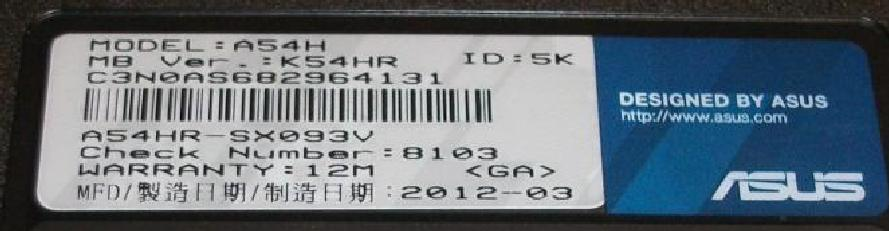
\includegraphics[width=0.4\linewidth]{pics/label1}};
%							\label{fig:label1}
%					\end{tikzpicture}
				\item impacchettare con cura ed etichettare i plichi;
				\item \textbf{cercare password, PIN, appunti;}
				\item valutare la necessità di rilievi dattiloscopici.
			\end{itemize}		
		In questa fase inizia la \textit{catena di custodia} del materiale fisico.
		\begin{figure}
			\centering
			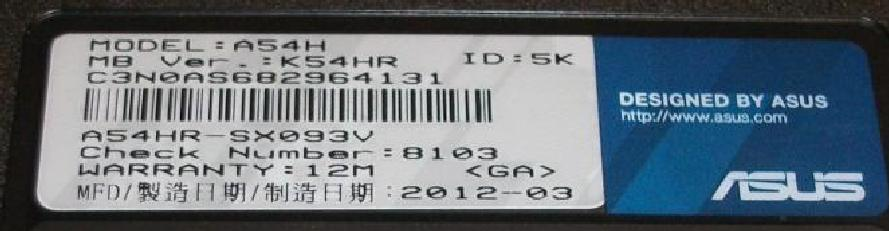
\includegraphics[width=0.6\linewidth]{pics/label1}
			
			\label{fig:label1}
		\end{figure}

			
	\end{frame}
	
	\begin{frame}
		\frametitle{Si può obbligare qualcuno a rivelare una password?}
		
		Nel corso della perquisizione potrà essere chiesto di rivelare password, PIN o altre informazioni utili per accedere ai dati.
		\vfill
		La P.G. è tenuta ad informare sul diritto a non rispondere di cui agli artt. 60 co. 3 e 350 c.p.p., altrimenti il dato ottenuto sarà \textbf{inutilizzabile}.
		\vfill
		\centering
		\Large\textbf{``Nemo tenetur se detegere''}
		
		\scriptsize(nessuno può essere obbligato ad autoaccusarsi)
		
	\end{frame}
	
	\begin{frame}
		\frametitle{Caso 2: computer acceso}

		Come procedere:
		\begin{itemize}
			\item \textbf{non staccare subito la spina:} si perderebbero dati preziosi;
			\item visualizzare ``a mano'' finestre aperte, pagine web attive, processi, ecc. o con apposito software;
			\item documentare tutta l'attività svolta sul computer, anche filmando il monitor e registrando una nota vocale che descriva le operazioni (come nei film americani!). 
			
		\end{itemize}
		\vfill
		\textit{Ogni atto svolto con queste modalità è di natura irripetibile!}

		\vfill
		Terminate le operazioni di \textit{``live forensic''} si può spegnere il dispositivo: \textbf{staccando la spina e MAI effettuando la procedura di arresto prevista dal sistema operativo!}
	\end{frame}
	
	\begin{frame}
		\frametitle{Sincronizziamo gli orologi}
		Qualora si operi su un dispositivo acceso, vanno sempre annotate l'ora e la data correnti del sistema, rapportandole a quelle effettive dell'intervento.
		\begin{figure}
			\centering
			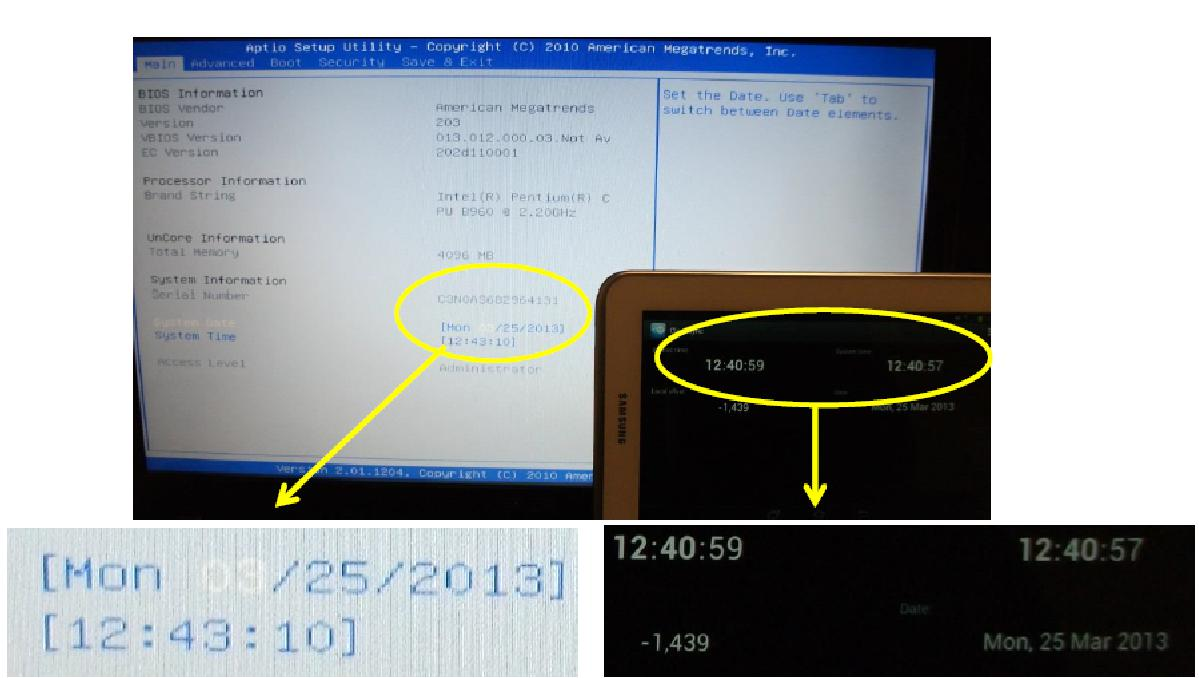
\includegraphics[width=0.6\linewidth]{pics/dataora}
			\label{fig:dataora}
		\end{figure}
		Questo è di fondamentale importanza per mettere in relazione gli orari delle operazioni della P.G. con i dati che verranno estratti dall'analisi \textit{post mortem}.
	\end{frame}
	
	\begin{frame}
		\frametitle{Caso 3: server o apparecchiatura di rete}
		
		Come mettere in sicurezza dati conservati su un server:
		
		\begin{itemize}
			\item capire se l'apparecchiatura in questione sia o meno nella completa disponibilità dell'indagato;
			\item limitare i ``danni collaterali'' provocati a persone non coinvolte nell'attività dell'indagato;
			\item se non è presente un tecnico, affidarsi all'amministratore del sistema per estrapolare al meglio il materiale di interesse.
			
		\end{itemize} 		
		Sequestrare tutto per poi scremare \textit{a posteriori} può andare bene per i computer  di una privata abitazione: fermare l'attività di un'azienda, incolpevole delle attività criminali degli utenti, dimostra una mancanza di professionalità. 
		\vfill
		\textbf{Non dimenticare mai che più materiale viene sequestrato, più dati si devono analizzare!}
		
	\end{frame}
		
	\section[Disp. mobili]{Dispositivi mobili}
	\begin{frame}
		\frametitle{Come operare sui dispositivi mobili}
		I dispositivi mobili sono sempre più simili a computer che non a semplici dispositivi di comunicazione quali erano i ``vecchi'' cellulari: ormai, infatti, \textit{smartphone} e \textit{tablet} hanno capacità di archiviazione tra i 32 o 64 GB dei modelli di punta e i 4-8 GB dei modelli più economici. Possono contenere moltissime informazioni e il loro uso pervasivo fa si che, molto più del PC di casa, siano la principale piattaforma di archiviazione dati degli utenti.
		\vfill
		Le modalità di sequestro di tali apparati necessitano a loro volta di alcuni accorgimenti particolari e richiedono un minimo di preparazione da parte degli operatori.
	\end{frame}
	
	\begin{frame}[shrink]\label{frame:Dispositivo_mobile_acceso}
		\frametitle{Dispositivo acceso}
		Per spegnerlo è necessario staccare la batteria: questa operazione spesso comporta la perdita delle informazioni volatili, per cui è necessario annotare (se possibile):
		\begin{itemize}
			\item l'attività in corso;
			\item ora e data del \textit{device} in rapporto a quelle reali;
		\end{itemize} 
		
		In caso di urgenza, potrebbe essere utile visualizzare le ultime chiamate effettuate e ricevute, consultare la rubrica e leggere eventuali SMS o MMS ricevuti. Nel fare ciò, attenzione a:
		\begin{itemize}
			\item non effettuate per nessun motivo chiamate;
			\item non spostare il dispositivo (per evitare di cambiare la cella agganciata).
		\end{itemize}
		
		Per ovviare al problema delle celle e delle chiamate, si dovrebbe inserire il dispositivo in una \textit{gabbia di Faraday} che impedisca che esso si colleghi alla rete mobile, che però raramente è a disposizione della P.G. operante.
	\end{frame}
	
	\begin{frame}
		\frametitle{Dispositivo spento}
		\begin{itemize}
			\item non accendere mai gli apparecchi rinvenuti spenti;
			\item cercare e sequestrare SIM card e schede di memoria contenute nel telefono, annotando numeri di serie e altri dati utili;
			\item cercare i codici di accesso al telefono (PIN, PUK e altro);
		\end{itemize}
		
		\begin{figure}
			\centering
			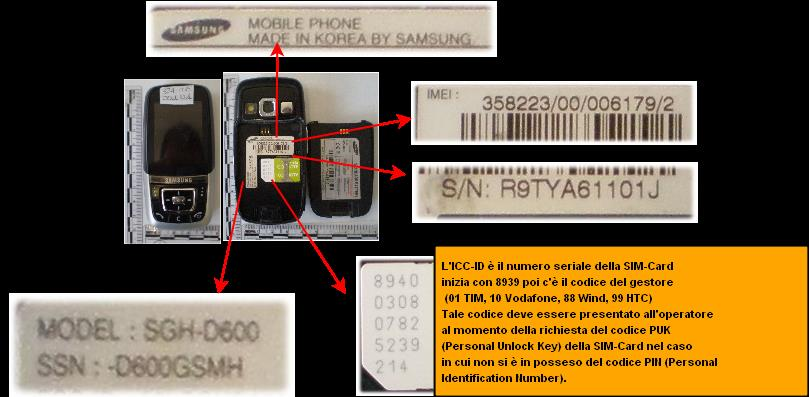
\includegraphics[width=0.4\linewidth]{pics/samsung_example}
			\label{fig:samsung_example}
		\end{figure}
				
		Nel caso sia necessario rimuovere la batteria, ricordiamo che ciò spesso azzera la memoria volatile: si deve valutare la priorità e l'importanza delle informazioni ricercate.
	\end{frame}
	
	\begin{frame}
		\frametitle{Le analisi forensi sugli \textit{smartphone}}
		\centering 
		
		\textbf{Le analisi forensi sui telefoni di nuova generazione sono generalmente non ripetibili.} 
		\vfill
		\justifying
		Per effettuare la copia forense (che non è nemmeno sempre possibile) di terminali Android o iOS (Apple iPhone e iPad) è necessario installarvi un apposito software dopo aver effettuato il \textit{rooting} o il \textit{jailbreak} del dispositivo. 
		\vfill

		Si deve \textbf{modificare} il contenuto della memoria, alterando la prova! 
		\vfill
		\centering
		\textbf{\'{E} evidente che ciò non è ``forensically sound''.}
	\end{frame}		
	
	\section{Analisi forense}
	
	\begin{frame}
		\frametitle{I principi dell'analisi forense}
		\begin{enumerate}
			\item \textbf{Tracciabilità della catena di custodia (\textit{chain of custody}) dei reperti}: ogni passaggio di mano, ogni apertura dei plichi sigillati, ogni operazione svolta deve essere registrata.
			\item \textbf{Integrità dei dati}: in nessun momento dell'analisi devono essere in alcun modo modificati i dati contenuti nei reperti.
			\item \textbf{Verificabilità e ripetibilità di tutte le operazioni svolte}: chiunque deve essere in grado di riprodurre, avendo gli strumenti adeguati, le operazioni svolte nell'analisi ottenendo gli stessi risultati.
		\end{enumerate}

	\end{frame}
	
	\begin{frame}
		\frametitle{Competenze necessarie per l'analisi forense}
		
		\begin{enumerate}
			\item Concetto di memoria volatile e persistente.
			\item Architettura hardware di un computer.
			\item Concetto di BIOS.
			\item Concetto di periferiche e memorie di massa.
			\item Concetto di \textit{hash}.
			\item Architettura base dei sistemi operativi Microsoft (cartelle utente e di sistema, file di log, file temporanei, registro).
			\item Architettura base dei sistemi Apple (idem).
			\item Funzionalità base dei sistemi GNU/Linux (soprattutto per l'utilizzo dei tool per il ``\textit{live forensic}'').
			
		\end{enumerate}
		
	\end{frame}
	
	\begin{frame}
		\frametitle{Non tutti gli informatici sono esperti forensi}
		\begin{center}

		\textbf{\`{E} sufficiente un buon informatico per fare una analisi forense?}
		
		Non sempre...
		\end{center}
		
		Un buon esempio è il referente telematico: per quanto bravo, non necessariamente conosce i principi base dell'analisi forense. 
		
		Anche sedicenti esperti informatici esterni spesso non sono affatto tali in ambito forense.
		
	\end{frame}
	
	\begin{frame}
		\frametitle{I software per l'analisi forense}
		\begin{enumerate}
			\item Software commerciali:
			\begin{itemize}
				\item \textbf{EnCase Forensic} della Guidance Software (\textit{computer forensic});
				\item \textbf{UFED} della Cellebrite (\textit{mobile forensic});
				\item \textellipsis
			\end{itemize}
			\item Software liberi (basati su GNU/Linux):
			\begin{itemize}
				\item \textbf{CAINE} (\textbf{C}omputer \textbf{A}ided \textbf{IN}vestigative \textbf{E}nvironment), distribuzione italiana, relativamente facile da utilizzare e completa;
				\item \textbf{DEFT} (\textbf{D}igital \textbf{E}vidence \& \textbf{F}orensic \textbf{T}oolkit), distribuzione italiana completa e aggiornata;
				\item molte altre distribuzioni di GNU/Linux concepite per le esigenze degli investigatori forensi, alcune dedicate a specifici settori quali l'analisi e l'acquisizione di computer Apple, dispositivi mobili o altre particolarità.
			\end{itemize}
		\end{enumerate}
	\end{frame}
	
	
	\begin{frame}
		\frametitle{Pregi del software libero [1/2]}
		La più interessante caratteristica delle distribuzioni GNU/Linux citate (CAINE e DEFT) è quella di poter essere masterizzate su un CD/DVD o eseguite direttamente da chiavetta USB, permettendo di operare sul posto \textbf{con la certezza di accedere ai dati in sola lettura} senza comprometterne l'integrità. 
		
		Avendone la possibilità (e i supporti per il riversamento), si può procedere direttamente alla copia forense \textit{on the fly} delle memorie di massa.
		
	\end{frame}
	
	\begin{frame}
		\frametitle{Pregi del software libero [2/2]}
		\framesubtitle{Una questione di controllo e di etica}
		
		In ogni settore, la pubblica amministrazione e in particolare le forze di polizia dovrebbero, per quanto possibile, tendere all'utilizzo di software libero (a sorgente aperto).
		\vfill
		Questo, oltre a ridurre i costi, dà il controllo completo sulle funzionalità e permette di verificare, in ogni momento, se il software si comporta nel modo corretto.
		\vfill
		Il software libero è pubblicato sotto i termini di una licenza libera, ovvero che ne incoraggia l'utilizzo, lo studio, la modifica e la redistribuzione.
		
	\end{frame}
	
	\begin{frame}
		\frametitle{Software commerciale o libero?}
		Che si usi uno strumento o un altro, l'aspetto fondamentale è l'indipendenza del risultato ottenuto dallo strumento utilizzato per ottenerlo: per quanto il software commerciale sia elaborato e sofisticato, gli stessi risultati si possono ottenere con software libero.
	\end{frame}
	
	
	\begin{frame}
		\frametitle{La copia forense [1/2]}
		Prima ancora di iniziare a analizzare il contenuto di un computer o comunque di un dispositivo digitale con al suo interno dei dati immagazzinati, è necessario effettuarne una \textbf{copia forense}.
		
		\vfill
		La copia forense (o bit-stream image), nel lessico forense, indica l'acquisizione di documenti in formato digitale che genera una copia bit a bit da un dispositivo di memoria di massa a un altro.\cite{wiki:Copia_forense}
		
		\vfill
		
		Essa comporta la duplicazione di tutte le zone del disco, anche quelle che non contengono alcun file direttamente visibile all'utente, definite tecnicamente aree non allocate -- ovvero i file cancellati.
			
	\end{frame}
	
	\begin{frame}[shrink]
		\frametitle{La copia forense [2/2]}
		Effettuare un copia forense necessita di un accorgimento tecnico fondamentale: \textbf{la protezione in scrittura del disco da copiare.}
		
		Per ottenerla ci sono due possibilità:
		\begin{itemize}
			\item un dispositivo che faccia il blocco a livello hardware;
			\item una workstation con a bordo un sistema operativo pensato per le analisi forensi.
		\end{itemize}
		
		\begin{figure}
			\centering
			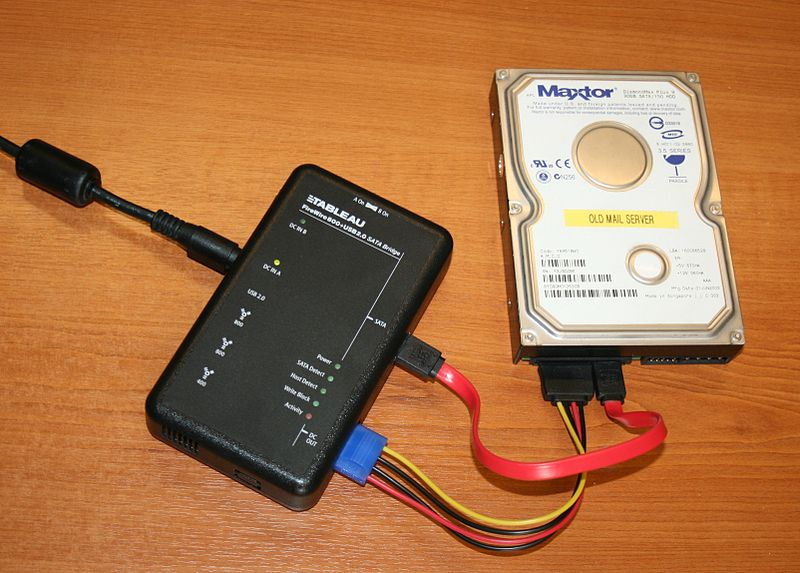
\includegraphics[width=0.25\linewidth]{pics/800px-Portable_forensic_tableau}
		
			\label{fig:800px-Portable_forensic_tableau}
		\end{figure}
		Quello che \emph{non si deve fare} è collegare il disco da copiare al proprio computer e ``trascinare le cartelle'' da un'altra parte -- già solo collegandolo ad un computer non predisposto per l'analisi forense, ci sto scrivendo informazioni, ``sporcando'' la prova.
				
	\end{frame}
	
	\begin{frame}
		\frametitle{Hash, l'impronta digitale elettronica [1/2]}
		Una volta effettuata la copia -- o immagine -- forense è indispensabile procedere al calcolo dell'\textit{hash}.
		\vfill
		La generazione dell'\textit{hash} di una evidenza forense è estremamente importante ed è la prova dell'integrità dei dati acquisiti: chiunque si approccia all'analisi dei dati effettua, per prima cosa, il calcolo dell'\textit{hash}: se esso differisce da quello calcolato i sede di acquisizione, il secondo perito non procederà con il lavoro ed eccepirà l'integrità del dato. Infatti, una modifica ancorché minima del contenuto di una evidenza digitale farà sì che l'impronta risultante sarà completamente diversa.
	\end{frame}
	
	\begin{frame}
		\frametitle{Hash, l'impronta digitale elettronica [2/2]}
		
		La funzione di hashing è \textit{non iniettiva}, quindi non reversibile e la probabilità di collisioni (ovvero di due serie di dati che forniscano la stessa sequenza di bit) è estremamente remota (per quanto non impossibile) ed è inversamente proporzionale alla complessità dell'algoritmo di calcolo.
		
		
		\begin{table}
			\scriptsize
			\centering
			\begin{tabular}{c|c|c}
				
				Stringa & Tipo di \textit{hash} & valore \\
				\hline
				\multirow{2}{*}{\texttt{Carabinieri}} 
				& \texttt{MD5} & \texttt{dae05abfa4bfb7d7adcc696ee55a38de} \\
				\cline{2-3}
				& \texttt{SHA1} & \texttt{88df4a0528da6b42987bd6542ee8d1d9f9457ec7} \\
				
				\hline
				\multirow{2}{*}{\texttt{carabinieri}}
				& \texttt{MD5} & \texttt{30ef5966704603d09f86bf35f2005e48} \\
				\cline{2-3}
				& \texttt{SHA1} & \texttt{2db401a3d74fe36b974de779be8c5b726a2de64c} \\
			\end{tabular}
			
		\end{table}
		
		L'\textit{hash} può essere effettuato su qualsiasi dato, sia esso un singolo file o l'immagine di una partizione o di un disco.
	\end{frame}
	
	\begin{frame}
		\frametitle{Sequenza delle operazioni preliminari all'analisi}
		
		\begin{enumerate}
			\item verifica dell'integrità fisica dei reperti;
			\item individuazione delle memorie di massa;
			\item disconnessione fisica delle memorie di massa dai dispositivi;
			\item collegamento delle memorie di massa al sistema di analisi forense -- se possibile tramite un \textit{write blocker} fisico;
			\item clonazione dell'evidenza digitale su un supporto apposito;
			\item generazione dell'\textit{hash} del dispositivo sorgente e dell'immagine generata e confronto dei risultati;
			\item sigillatura e archiviazione dei dispositivi originali;
			\item copia di lavoro dell'immagine acquisita;
			\item archiviazione della prima copia, a disposizione dell'A.G. e delle eventuali ulteriori perizie di parte o del P.M.;
			\item analisi della copia di lavoro.
		\end{enumerate}
		
	\end{frame}
	
	\begin{frame}[allowframebreaks]
		\frametitle{Cenni sull'analisi forense}
		Le fasi della generica analisi forense sono sinteticamente elencate di seguito. L'opportunità di svolgerle tutte, nell'ordine che di volta in volta si ritiene più opportuno, va valutata sulla base di ciò che cerca. 

		\textbf{L'elenco non è e non vuole essere completo.}
		
		
		\begin{itemize}
			\item analisi del contenuto della ``S.M.A.R.T. area''  del disco rigido, qualora presente, al fine di avere informazioni sull'età del disco e su eventuali ipotizzabili sostituzioni recenti dello stesso;
			\item annotazione del software di base rinvenuto installato sul supporto di memoria, con particolare riferimento alla configurazione del Sistema Operativo;
			\item valutazione della dimensione ed analisi del contenuto della ``Unused Disk Area'';
			\item recupero delle ``cartelle orfane'' ed analisi dei file in esse indicizzati;
			\item analisi delle cartelle e dei file rinvenuti cancellati;
			\item analisi dell'area di memoria non allocata per ciascuna partizione rilevata sul supporto;
			\item rilevazione di eventuali file con estensione alterata;
			\item analisi storica delle date di creazione, modifica, ecc. dei file;
			\item ricerca di specifici contenuti testuali;
			\item visualizzazione dei file contenenti immagini fotografiche;
			\item visualizzazione dei file contenenti materiale audiovisivo;
			\item analisi dei file di archivio compressi;
			\item analisi della posta elettronica rinvenuta archiviata;
			\item analisi delle tracce della navigazione in Internet;
			
		\end{itemize}
	\end{frame}
	
	\section{Live forensic}
	
	\begin{frame}
		\frametitle{Perchè operare \textit{live}}
		Fino a qualche anno fa, in presenza di un computer acceso, si diceva di spegnerlo brutalmente e repertarlo.
		\vfill
		Lo spegnimento forzato di una macchina attiva determina perdite di dati, principalmente di quanto contenuto nella RAM: si riteneva che il costo di queste perdite fosse molto basso rispetto al rischio di far interagire un profano con la macchina per ottenere direttamente informazioni, riducendo al minimo la sovrascrittura dei dati sulle memorie di massa attive.
		\vfill
		A volte, però, i dati volatili sono estremamente importanti e gli operatori dovrebbero saperli assicurare.
	\end{frame}
	
	\begin{frame}
		\frametitle{Quando operare \textit{live}}
			Molte delle possibili prove presenti nella memoria RAM non vengono registrate sui supporti persistenti. Tra i motivi che possono indirizzare verso l'approccio \textit{live} possiamo menzionare:
			
			\begin{enumerate}
				
				\item{\textbf{comunicazioni con dati non persistenti,}} come le chat, che nello spegnimento forzato vengono completamente perse;
				\item{\textbf{crittografia}}: dopo lo spegnimento del sistema, l'accesso a partizioni criptate può risultare complicata se non impossibile, richiedendo di solito l'immissione di una password o di una passphrase;
				\item{\textbf{server:}} per grandi sistemi l'idea di spegnerli per repertarli è frutto solo dell'ignoranza;
				\item{\textbf{necessità}} di analizzare qualsiasi servizio o applicazione attivo sulla macchina.
			\end{enumerate}
	\end{frame}
	
	\begin{frame}
		\frametitle{Limiti dell'analisi \textit{live}}
		Se si ammette la possibilità di interagire sulla scena del crimine con la macchina, si accetta che:
		\begin{itemize}
			
			\item il repertamento dei dati sia parziale e incompleto;
			
			\item alcuni dati di interesse possano emergere durante l'interazione con la macchina per cui il repertamento avviene a fasi incrementali;
			
			\item preparazione ed analisi siano ridotti al minimo durante l'interazione con il sistema per diminuire la possibilità di causare cambiamenti importanti nelle memorie digitali in analisi e lasciare la parte approfondita di essi all'approccio statico;
			
			\item il \textit{reporting} non sia quello del \textit{forensic} statico, che si propone di spiegare le operazioni in dettaglio e presentarle in dibattimento.
			Si tratta di una sorta di perquisizione;
			
			\item \textbf{l'attività sia irripetibile}.
			
		\end{itemize}
	\end{frame}
	
	\begin{frame}
		\frametitle{A proposito di irripetibilità}
		
		Essa è:
		\begin{itemize}
			
			\item \textbf{di natura tecnica:} non esiste infatti possibilità di realizzare analisi e repertamento dati live senza modificare almeno una parte della memoria del sistema.
			
			\item \textbf{di natura temporale:} la situazione della macchina all'atto dell'attività è frutto del momento e la sua complessità è tale da non poter essere riprodotta.
			
			\item \textbf{relativa all'osservabilità:} lo stato di un computer reperto attivo, in tutte le sue variabili, non è completamente osservabile perché la sonda che si dovrebbe inserire per compiere tale osservazione andrebbe a modificarne proprio lo stato.
			\end{itemize}
	\end{frame}
	
	\begin{frame}[shrink]
			\frametitle{Uno strumento per il \textit{live forensic}}			
			\textbf{Win-UFO} (\url{http://win-ufo.org/about.shtml}) è un software libero che può essere installato su una chiavetta USB da inserire nel computer oggetto dell'attività \textit{live} e permette di estrapolare e salvare dati relativi allo stato di funzionamento della macchina sulla quale viene fatto girare.
			
			\begin{figure}
				\centering
				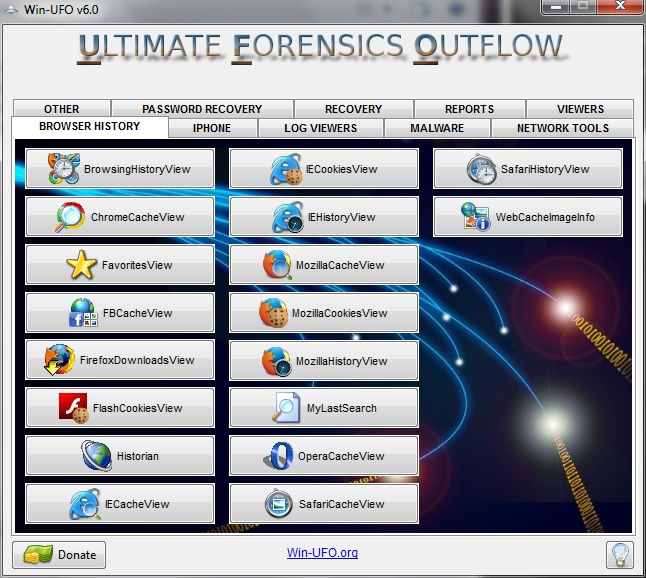
\includegraphics[width=.4\linewidth]{pics/winufo1}
						
			\end{figure}

			
	\end{frame}
	
	\begin{frame}
		\frametitle{Pro e contro del \textit{live forensic}}
	Pro:
	\begin{itemize}
		\item i dati forensi raccolti in un sistema live possono produrre prove che non emergerebbero in sede di analisi \textit{post mortem};
		\item buona velocità di esecuzione (cosa che magistratura e legali apprezzano).
	\end{itemize}
	\vfill
	Contro:
	\begin{itemize}
		\item standard in evoluzione;
		\item pochi precedenti legali;
		\item rischio di contaminazione delle prove;
		\item non sempre magistrati e avvocati comprendono la problematica;
		\item \textbf{procedimento assolutamente irripetibile}.
	\end{itemize}

	\end{frame}
	
	\begin{frame} %mettiamola per ultima questa
		\frametitle{La ``perquisizione informatica''}
		In alcuni, specifici casi, è possibile accendere un dispositivo spento senza strumenti forensi per verificare il contenuto. 
		\vfill
		Si può parlare di perquisizione informatica:
		\begin{itemize}
			\item è attività tipica (art. 352 c.p.p);
			\item è accertamento tecnico non ripetibile e richiede la presenza del difensore (360 c.p.p.);
			\item \textbf{deve essere concordata con il magistrato di turno.}
		\end{itemize}
	\end{frame}
	

	
	\begin{frame}[shrink]
		\frametitle{Perquisizione informatica: un esempio}
		Per decidere se sequestrare o meno un portatile (reato ipotizzato: \textit{truffa tramite la stampa di assegni falsi}), si è proceduto alla perquisizione informatica con la presenza del legale.
		\vfill
		Tra i ``\texttt{Documenti recenti}'' era presente il file ``\texttt{seriale\_f.psd}'' che però rimandava a una chiavetta USB e quindi non era accessibile.
		\vfill
		Il nome del file era interessante e suggestivo e sufficiente per il sequestro. In sede di analisi tra i file cancellati si è trovato proprio un assegno!
		\begin{figure}
			\centering
			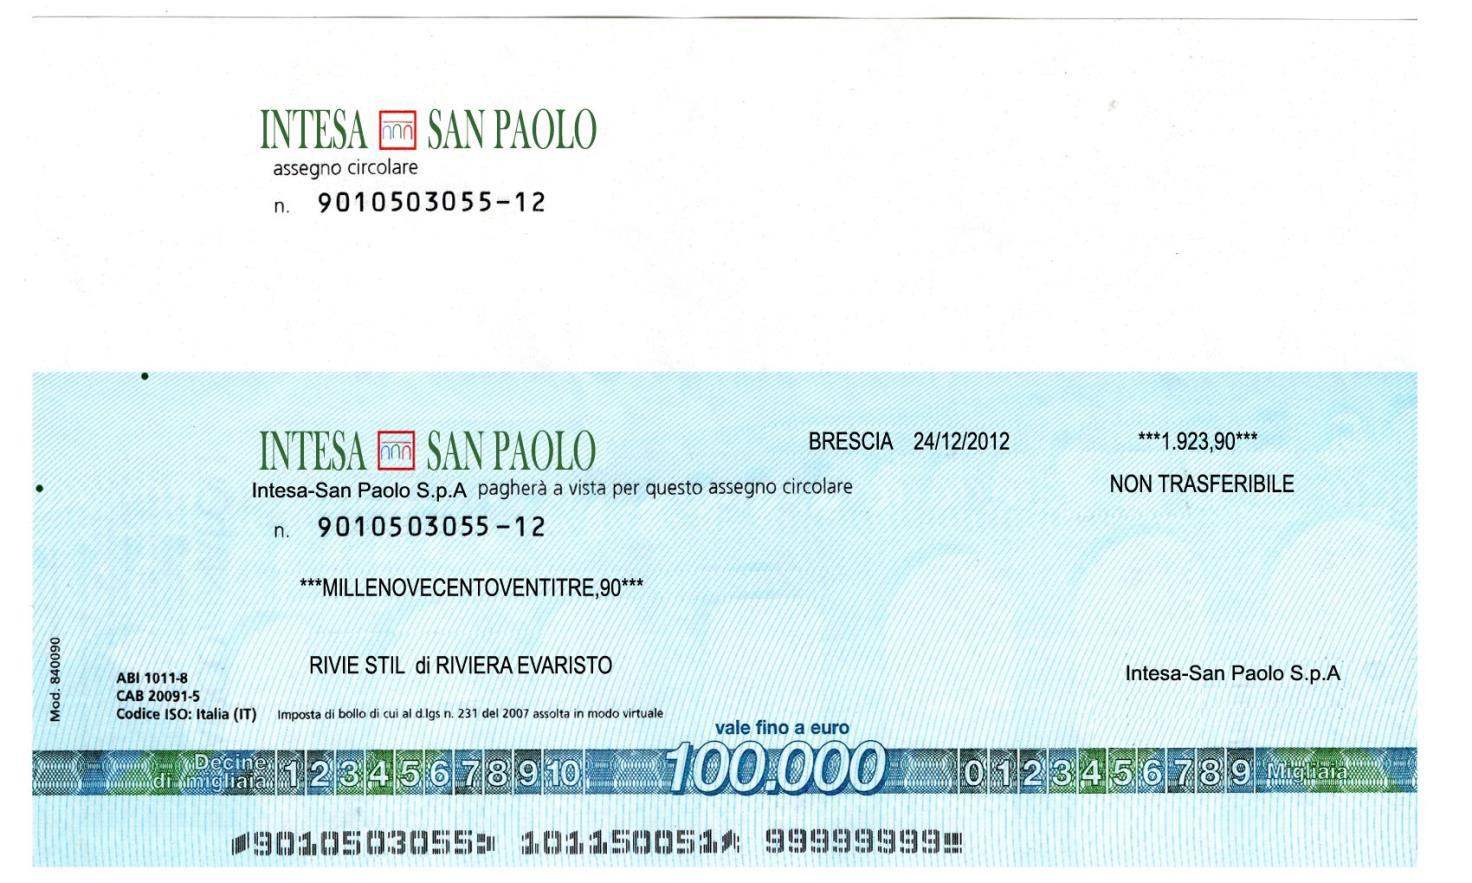
\includegraphics[width=0.6\textheight]{pics/assegno_psd}
			\label{fig:assegno_psd}
		\end{figure}
	\end{frame}
		
	
	
	\section*{}	
	\begin{frame}
		\vfill
		\centering
		\Large Grazie per l'attenzione.
		\vfill
		\huge Domande?
		\vfill	
		\tiny \textbf{Nota:} questa presentazione \textbf{non} è stata realizzata con Microsoft~Powerpoint\textsuperscript\textcopyright bensì con \textsf{\LaTeX}.
	\end{frame}
	
	\begin{frame}
		\frametitle{Riferimenti}
		\tiny
		\bibliographystyle{plain}
		\setbeamertemplate{bibliography item}{\insertbiblabel}
		\bibliography{forensics}
	\end{frame}
\end{document}